\documentclass[11pt]{article}

\usepackage[utf8]{inputenc}
\usepackage[english]{babel}
\usepackage{sectsty}
\usepackage{listings}
\usepackage{graphicx}
\usepackage{wrapfig}
\usepackage[backend=biber,style=authoryear-icomp]{biblatex}
\usepackage{caption,subcaption}
\usepackage[scaled]{helvet}
\usepackage{csquotes}
\usepackage{listings}
\usepackage{xcolor}
\usepackage{datetime}

%headers and footer
\usepackage{fancyhdr}

\usepackage{blindtext}
\renewcommand{\subsectionmark}[1]{\markright{\thesubsection\ #1}}

\pagestyle{fancy}
\fancyhf{}
\fancyfoot[C]{\thepage}
\fancyhead[C]{I Know You!}
\fancyhead[R]{Nicolà Lohr}
\fancyhead[L]{\nouppercase{\leftmark}}
\fancyheadoffset[R,L]{0cm}
\renewcommand{\headrulewidth}{0.5pt}

%formating
\usepackage{calc}
\setlength\textwidth{7in}
\setlength\textheight{9in}
\setlength\oddsidemargin{(\paperwidth-\textwidth)/2 - 1in}
\setlength\topmargin{(\paperheight-\textheight-\headheight-\headsep-\footskip)/2 - 1in}

\lstset{language=Python} 

%\usepacket{geometry}
%\geometry{ a4paper, total={170mm,257mm}, left=20mm, top=20mm, }

\definecolor{codegreen}{rgb}{0,0.6,0}
\definecolor{codegray}{rgb}{0.5,0.5,0.5}
\definecolor{codepurple}{rgb}{0.58,0,0.82}
\definecolor{backcolour}{rgb}{0.95,0.95,0.92}

\lstdefinestyle{python}{
   language=python,
   basicstyle=\small\fontencoding{T1}\ttfamily,
   captionpos=b,
   numbers=left,
   numbersep=5pt,
   numberstyle=\tiny\color{codegray},
	backgroundcolor=\color{white},   
    commentstyle=\color{codegreen},
    keywordstyle=\color{magenta},	
	stringstyle=\color{codepurple},
}
\lstdefinestyle{php}{
   language=PHP,
   basicstyle=\small\fontencoding{T1}\ttfamily,
   captionpos=b,
   numbers=left,
   numbersep=5pt,
   numberstyle=\tiny\color{codegray},
	backgroundcolor=\color{white},   
    commentstyle=\color{codegreen},
    keywordstyle=\color{magenta},	
	stringstyle=\color{codepurple},
}



\allsectionsfont{\centering \normalfont\scshape}

\linespread{1.5}
\setlength{\parindent}{0pt}
\setlength{\parskip}{8pt}

\addbibresource{sources.bib}
\defbibheading{online}{\subsection{Online-Quellen}}
\defbibheading{offline}{\subsection{Literatur}}


\title{\normalfont \normalsize \textsc{KSZ, Kantonsschule Zug} \\ [25pt]
\huge I Know You!\linebreak\linebreak \large Metadata Analysis \linebreak \large Appendix\\ 
}
\author{Nicolà Lohr\\[0.5cm]{\small Supervisor: Marco Schmid}}

\date{\normalsize\today}

\begin{document}

\clearpage
\newcommand{\HRule}{\rule{\linewidth}{0.5mm}}

\begin{center}


%\includegraphics[width=0.5\linewidth]{./kks.jpg}
\textsc{\Large  KSZ, Kantonsschule Zug}\\[0.8cm]

\vfill

% Title
\HRule \\[1.8cm]
\textsc{\Large  Wi-Fi metadata analysis}\\[0.8cm]
\textsc{ \huge  I Know You!}\\[0.4cm]
\textsc{Appendix}\\[1.4cm]

\HRule \\[1.5cm]

% Author and supervisor
\begin{minipage}[t]{0.38\textwidth}
\begin{flushleft} \large
\emph{Author:}\\
Nicolà Lohr \\ 


\end{flushleft}
\end{minipage}
\begin{minipage}[t]{0.6\textwidth}
\begin{flushright} \large
\emph{Supervisor:}\\
Marco Schmid
\end{flushright}
\end{minipage}

\vfill

% Bottom of the page
{\large \today}

\end{center}
\thispagestyle{empty}
\newpage
\thispagestyle{empty}
\newpage
\linespread{0.9}
\tableofcontents
\linespread{1.5}
\newpage

\section {School plan}
\begin{figure}
\centering
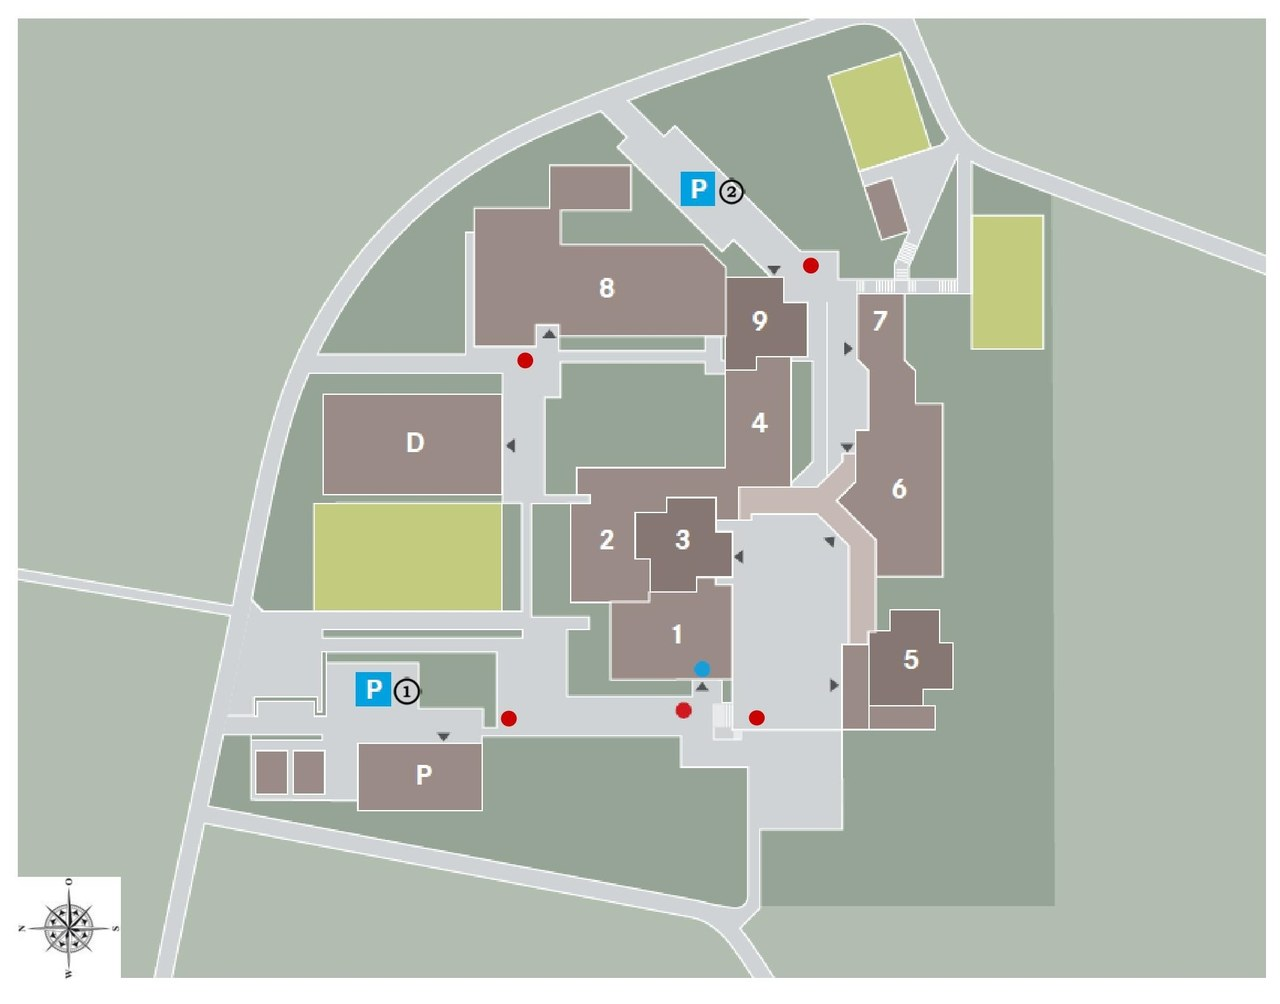
\includegraphics [width = \textwidth]{images/lageplan.jpeg}
\caption{The location plan of the KSZ\label{fig:locationplan}}
\end{figure}

For everyone that does not attend my school it is helpful to know where which building is.\footcite{kszlageplan} The numbers including P and D in the image are the building names. The blue point is the main entrance. I placed the WiFi Pineapple at the red point between building one and five. Most students arrive through the small path from the lower center, right passed the WiFi Pineapple.

\section{Definitions and Protocols}

\subsection{MAC-Address}
A MAC-address or short MAC is an unchangeable ID given by the manufacturer. It consists out of 48 bits split into six two-digit hexadecimal numbers, one byte. The MAC has to be unique in the world, otherwise the protocols will not work. 
Companies can buy the rights to the first three bytes and use all the variance of the other 3 bytes to give a unique ID to each device. Apple, for example, bought several of those, the one I got was 88:E9:FE. That is why I know if there is a device with the MAC of 88:E9:FE:11:22:33 it is an Apple device. This gives me the possibility to find out the phone or laptop brand by only this address. There are also ways to buy less MAC addresses if the company is not big enough. There were some attempts to guessing the model with only these bytes but with no real success.
\footcite{macaddress}
\subsection{Monitor-Mode}
Monitor-Mode, also known as RFMON (Radio Frequency Monitor), gives the computer the ability to capture Wi-Fi packets from the air, which are not meant for this computer. This is called sniffing. The devices are usually kind enough to only listen to the packet addressed to them and ignore the rest, but with monitor mode, it is possible to listen to every packet sent over the air.
Most standard Wi-Fi Cards lack the option to change into monitor mode because there is rarely any use of it. For the other cards there are many easy to use tools to change into the monitor mode. I used aircrack-ng and IP.

\footcite{monitor}
\subsection{Eduroam}
Eduroam is a secure, easy, and straightforward standard for Wi-Fi hotspots for schools and universities like at my school. The advantage is once signed in; one gets internet access as soon as in the range of an Eduroam hotspot. Eduroam is now available in over a hundred countries, and the organization behind the Eduroam provides many countries with fast and cheap Wi-Fi.\footcite{eduroam} Eduraom is based on the IEEE 802.1X protocol and uses RADIUS servers additionally as proxies to talk to other Eduroam RADIUS servers.\footcite[RADIUS Server]{WPA2} They do not share the information, they send the login to the right school which validates the username and password and sends back the corresponding response.\footcite{eduroam}

\subsection{WPA2-Enterprise}
WPA2-Enterprise is the system used for Eduroam. Difference from the WPA2-PSK, which is often used in private networks at home or restaurants, by a few significant points. First of all, WPA2-PSK only asks for a password, unlike in WPA2-Enterprise, where a username is requested as well. This makes it possible to differentiate the users of each other and therefore improve security with more significant amounts of devices connected. WPA2-Enterprise requires a validating server for Eduroam this is the RADIUS server, but there are alternative like Dot1x \footcite{radius}
This is a computer that authenticates every device trying to connect to the network. 802.1X is the policy that the authentication processed it based on. It comes in different systems named EAP. The security increases because the radius server authenticates each device before it connects. In this process, an encrypted tunnel can be created.
\footcite{WPA2}
The IT-department can find user which violated the policies. 

Recently WPA3 was released. Although it has some advantaged like authentication of the servers, it is nearly nowhere implemented. 

\subsection{IEEE 802.1x}
IEEE 802.1x is standard for port-based network access control (PNAC). It is used on wireless but also on wired networks. This system  controls the authentication of each user and device trying to access the network. It needs a supplicant to transform the authentication packages from the EAP negatiation to a form that the switch understandable packets. Most devices ave such a supplicants built in natively.There are companies which provide this supplicant to unsupported devices. 

It is used in WPA2-Enterprise and it the possibility to login in with personalized credentials. This is often seen in big companies, school and colleges. They use it because it gives them more control over which devices belongs to whom and what they searched from. Every time a devices tries to connect to the Wi-Fi or wired network it authenticates itself with the username and the password. If the user is validated the login is saved by a RADIUS server in the background (there are alternatives to RADIUS but this is the most common one).

With the information saved by the network the system can detect individual users and potential profiling of those. This could lead to a saver and faster network and access to the internet.\footcite{ieee802.1x}


\section{Technologies}
\subsection{Wi-Fi-Pineapple}
\begin{wrapfigure}{r}{7cm}
\centering
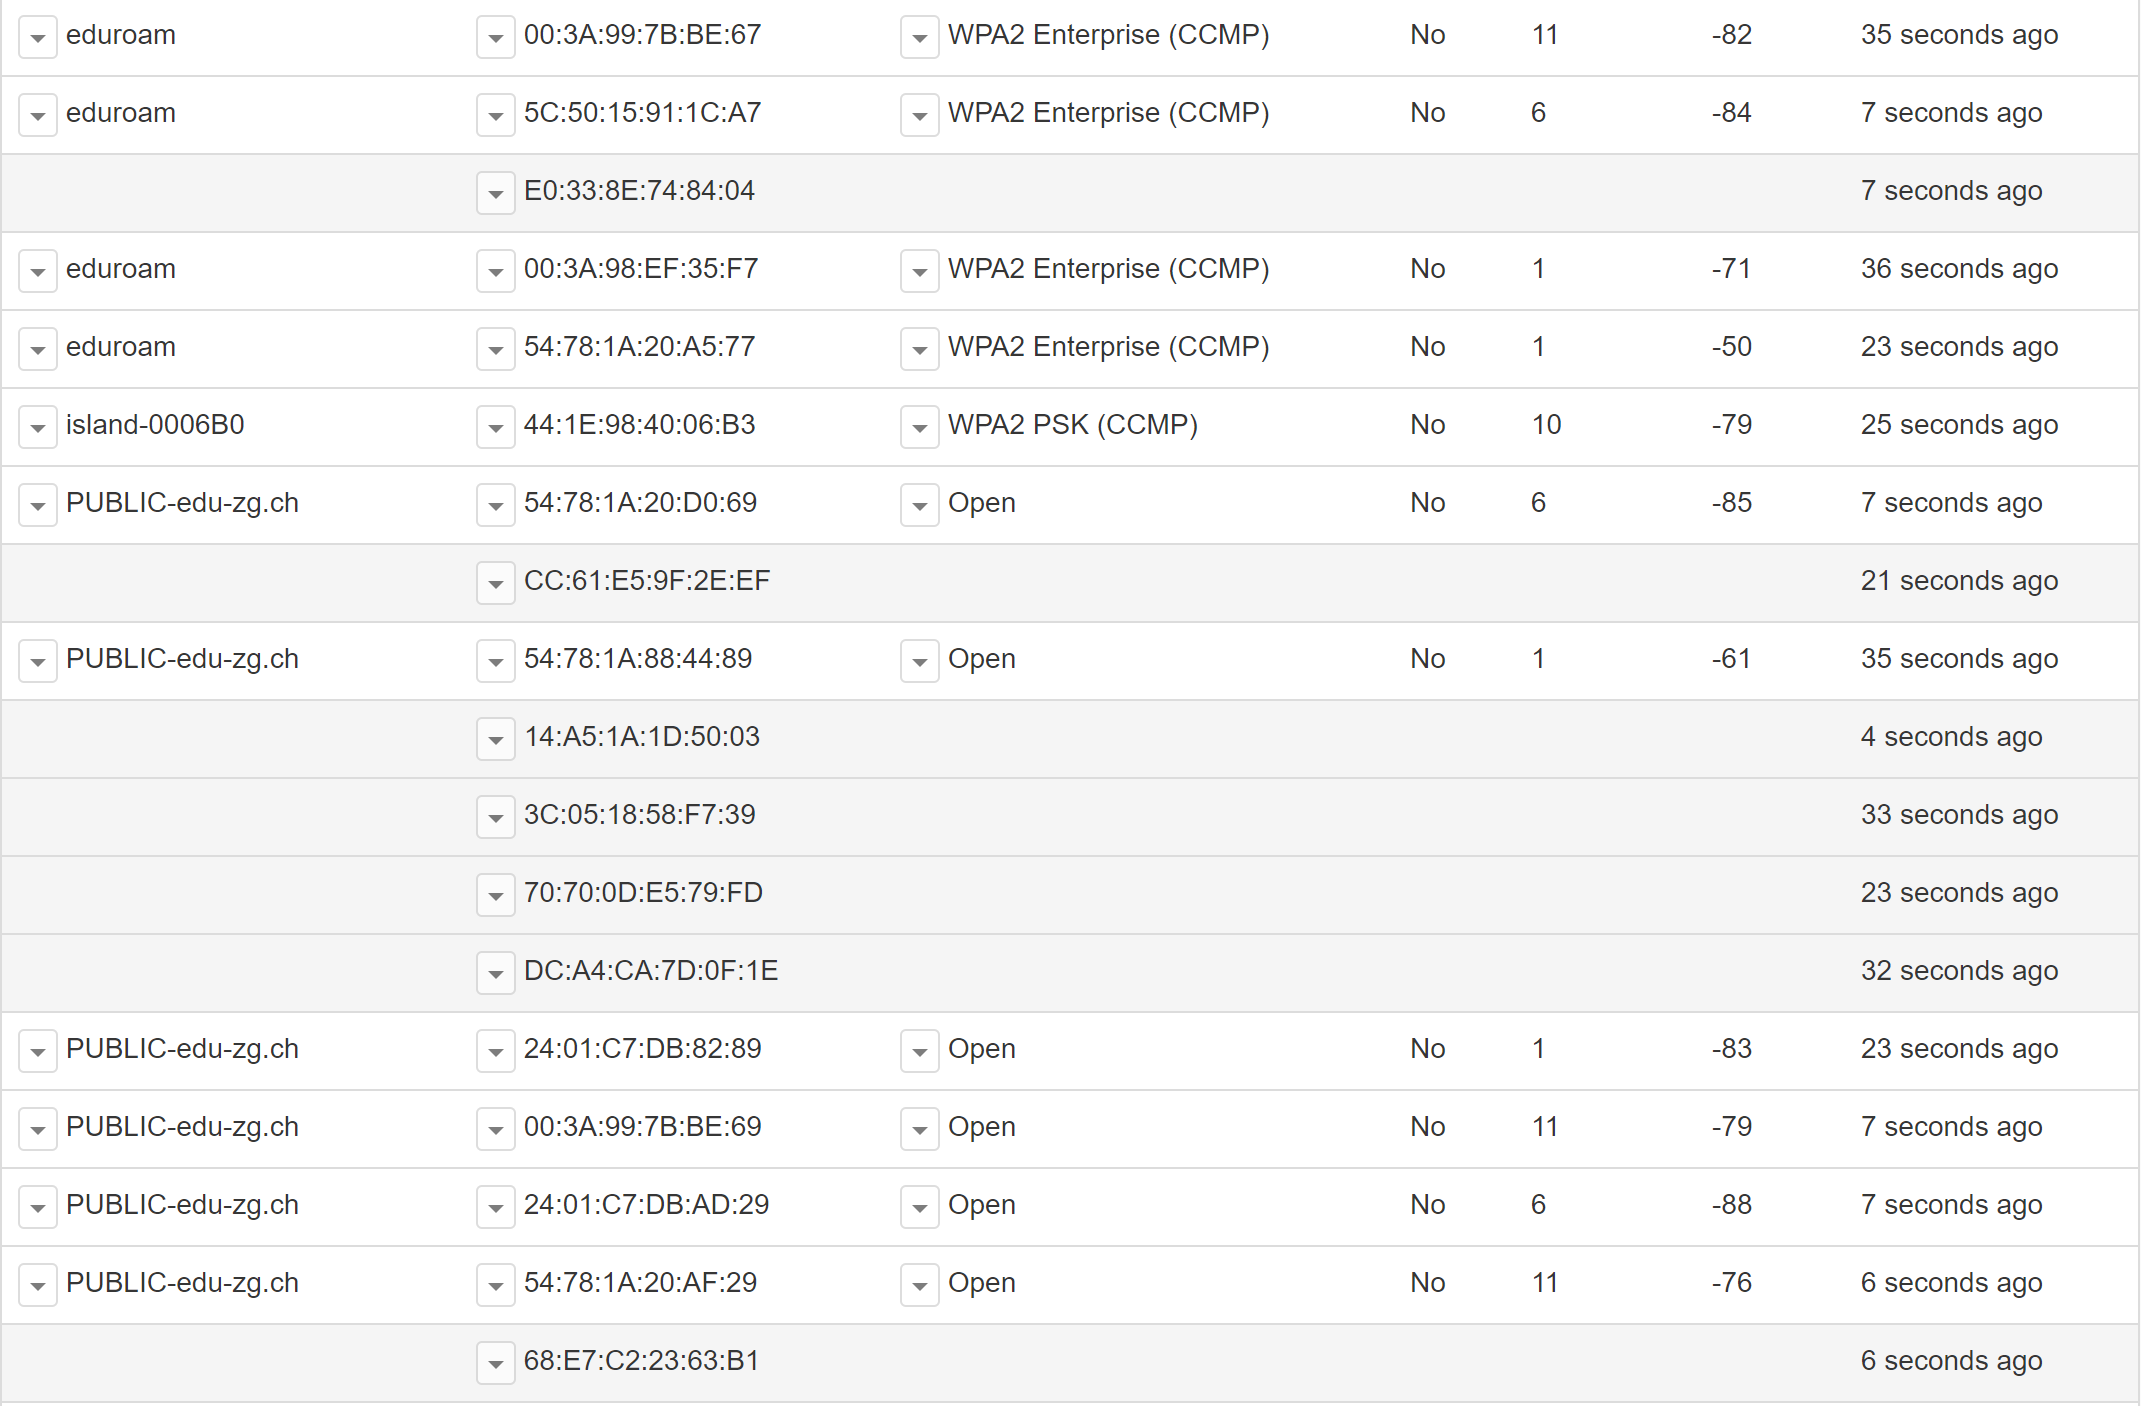
\includegraphics [width = 6cm]{images/example_wifi_pineapple.PNG}
\caption{Software image of the Wi-Fi pineapple\label{fig:wifi_pineapple}}
\end{wrapfigure}

The Wi-Fi-Pineapple is a small computer with a Linux operating system. It is optimized to capture Wi-Fi data in both 2.4 GHz and 5 GHz. It can also be used as a rogue access point and is generally looked at as one of the best penetration-testing toolkits for Wi-Fi. An rogue access point which pretends to be in another network than it is. It can perform active and passive attacks to find and analyze faults and vulnerabilities in the system.

Figure \ref{fig:wifi_pineapple} shows the software implemented in the WiFi pineapple. This is accessible through the website from the pineapple\footcite{wifipineapple}
\subsection{Ubertooth}
The Ubertooth is a device to sniff Bluetooth data similar then the Wi-Fi-pineapple does with Wi-Fi packets. It is an open-source wireless platform suitable for development and Bluetooth experiments. This device is one of the only affordable options to sniff Bluetooth packets and is available since 2010.
\footcite{ubertooth}
\section{Ideas behind the results}
\subsection{Class}

With my data, I filtered them just to the first and last data points each day. This helps stop bias from more or less data and reduces the calculation and distances the computer has to calculate. Another method to make it more consistent is that I reduced the data from multiple weeks to one single one. This is crucial to fill in the missing data points and create a standard amount of dimensions for later. If I had multiple reasonable values for one dimension, I could take the mean value of the ones I got. This minimizes the error rate because the random(more or less) distribution gives the possibility that I have one very late or early one. This excludes the maximum and the minimum. The average is still directly connected to the unfitting value. The mean, on the other hand, has the most promising result.

Tracking me for two weeks, I recognized I did not have enough data to make it fix for the ten dimensions. On Monday, it picked me up only in the afternoon, which does not make much sense. Apply advanced algorithms like KNN still gave me results. My result gave me the right class in the top ten.

This is not perfect, but a lot better than just guessing with my methods I needed more data. With a lot more data  (8 weeks) I finally had enough data to have nearly no missing data. This improved my result extremely.

If I removed the values which will not make sense (arriving in the afternoon or leaving before lunch) and calculated the distance there, I got surprisingly worse results.

Trying to optimize my result was hard.

A standard KNN algorithm finds the centroids in the N-Dimensional space given training data. The problem is that I do not have any training data. That is why I used the time-table as the centroids and calculated the distances between the points and the centroids. The best one wins. Because I did not divide the dimensions by the variance or standard variation (legitimate idea for weighting the different dimensions), I could use the exact times form the time table minus a descent constant (before and afterschool stay).



\subsection{Friends Tracking}
Like said in the paper, I used a simple counting method to find the friends who walk together. This system to run on my computer with all my data would have taken several centuries. I made a list of every MAC which appears on fifteen seconds of each other and used this list to move through all the data points. The inefficient part was that there were added to each other to count as friends. With optimizing this system only to add the new ones (needed a new list for that), I could reduce the running time by an important factor. It still took a while to run the program. The relative score between two MAC-addresses was the exciting part. If you have 30\% of your connections with one MAC, but this MAC has so many connections that you are only 1\% of its connections, then it is most likely a stationary machine or a tester. If the percentages are similar, I guess they are good friends. If a person has many people who have higher percentages, which this person as otherwise around it is fair to say, this person has many friends. The other way around you could consider someone with only a few connections with a high mutual percentage are good friends.
This method is more useful to use during the evening because in the morning it is very location-based. The same train arrives at a similar time, not necessarily friends.



\subsection{SBB}
This brings me to the train schedule. I used the same KNN algorithm then in classes, but this time I only checked at what time (only the minutes) the person arrives at school. If they arrive at 7:36 or 8:36 does not matter because the train regularly runs/ every hour. Of course, it can be late, and lately, that was often the case, but the mean value should still be decently representative. Estimating the walking time from the station to the school was not hard (8min), and with the online train schedule\footcite{sbbonlinefahrplan}, I could figure out the assumed arrival time of the students. I had the problem that some trains arrived at very similar times, but with just a few minutes difference, I could guess how they differ. With different arrival times, I calculated the distances between the different arrival times and the estimated train delivery. With this data, I was able to assume the living place of the people. I had no solutions for these results to compare them with. That is why I could not proof my results or validate them. This is also the reason why I had to use KNN.


\section{Code}
\subsection{Data Collection}
I got the data from the front port. I collected for multiple days and saved them in files that contain five minutes. The reason why I did not want just one file is 1.) Not enough ram for that much data, file corruption, when plugged out, 3) better overview.



\begin{lstlisting}[language=PHP, caption="Idea to put Wi-Fi card into monitor mode",style=php]
mount /dev/sda1 /mnt/
iw phy phy0 interface add mon0 type monitor 
ip l set up mon0 
tcpdump -i mon0 -w /mnt/file.pcap
\end{lstlisting}


\begin{lstlisting}[language=PHP,caption="Actual code used for the WiFi pineapple",style=php]
iw phy phy0 interface add mon0 type monitor
iw phy phy1 interface add mon1 type monitor
iw dev wlan0 del
iw dev wlan0-1 del
iw dev wlan1 del
ifconfig mon0 up
ifconfig mon1 up
iw dev mon0 set channel 1
iw dev mon1 set channel 100
mount /dev/sda1 /mnt/
tcpdump -G 300 -s 65535 -w /mnt/mon0\%s.pcap -i mon0 \&
tcpdump -G 300 -s 65535 -w /mnt/mon1\%s.pcap -i mon1 \&
\end{lstlisting}



The following code works if the tool aircrack-ng is installed...

\begin{lstlisting}[language=PHP, caption="aircrack-ng example"]
mount /dev/sda1 /mnt/
airmon-ng start wlan1
tcpdump -i wlan1mon -s 65535 -w /mnt/fileX.pcap
\end{lstlisting}




\subsection{Basic Proove of Conecpt}
There where a lot of different files which I had to read. Below it is shown how I read in the access point data. On each line, there is one new access point with its location. Going through all the lines and extracting the current MAC address and room was simple due to the repeating pattern in the file. I first thought of doing this with a REDEX, but this is not necessary here. As soon as all the information is gathered, it is saved in a dictionary for easy and fast access and, in the end, return in this dictionary.
Because the information is not written in an orderly faction I can use, I needed some external functions like radio\_MAC.
\begin{lstlisting}[language=Python, caption="read\_ap\_database\_type1",style=python]
def read_ap_database_type1(filename):
    aps = {}
    with open(filename, encoding='utf-8') as f:
        for ap in f.readlines():
            ap_info = ap.split(",")
            ap_mac = radio-mac(ap_info[0][1:17].upper())
            ap_room = ap_info[1].upper()[7:10]
            aps[ap_MAC.upper()] = ap_room
    return aps
\end{lstlisting}

Function radio\-MAC takes a MAC address given by access points, which was of my one bit. It invites the 4th bit in the 4th byte of the MAC address to make it match to the one in the log files.  For example  88:E9:FE:B2:7B:4 becomes  88:E9:FE:F2:7B:4. Note that in this example, the last number is missing due to the unimportant and unpredictability of it. For every access point, the MAC address the last digit is removed. 
After checking if the MAC has the correct length, the new value of the 4th byte is calculated with a simple XOR calculation. Before returning the MAC address, the new variable replaces the old one.
\begin{lstlisting}[language=python,caption="radio-mac",style=python]
def radio-MAC(file_mac):
    assert len(file_MAC)==16, f"unexpected length of mac: {file_mac}"
    new_value = hex_byte(int('40',16)^(int(file_MAC[9:11],16))) 
    new_mac = file_mac[:9]+new_value+file_MAC[11:]
    return new_mac
\end{lstlisting}

Other functions were needed to transform dec to hex and get the time in the right format.

For the time table and the log files, I had to do similar things. Notable is that one tries to minimize the amount of reading time and, if possible, store it in memory. This transaction gave me a speed boost of about 1'000.

I tried multiprocessing of the data, but the gain was too little that it was worth the time investment.

Finally, to track a person or more precise, a MAC address track\_MAC is the function to call. It requires the target MAC, the log filenames, the access point, and the time table. I purposely gave so many required variables, so it can be easier to modify. For a new year, change the time table or with more data change the filenames.
This function first calls another function. This function compares the log file with the access point positions to find out during which lessons you were in which rooms. With this information, it uses the time table to find out who had school during this lesson in this room and adds this to a list, which is returned to the track\_MAC function. With this result, it counts how many times which class appears in the list\_to\_percent function. All counted up the track\_MAC function returns the highest value, the one with the most overlapping from expected and realty. If there is no data found, it returns unknown.

\begin{lstlisting}[language=Python,caption="track-mac",style=python]
def track_mac(mac,filenames,aps,time_table_dic):
    classes=fit_to_lesson(filenames,aps,time_table_dic)
    dic = list_to_percent(classes[user_mac])
    if len(dic)!=0:
        return max(dic, key=dic.get), dic[max(dic, key=dic.get)]
    return "unknown", 0
\end{lstlisting}

This can be modified not only for one MAC address but to look for all. This takes a little longer but also finishes in a few minutes. 
The whole file can be imported into another python file and can be used. Every function returns aid if called with help(func).



\subsection{Advanced Proove of Conecpt}

Before I could do anything with Advanced Algorithms and my data, I had to get rid of the "pcap" file format. This file format is beautiful to look at in Wireshark but hard to work within python. There is a too called "scapy", which works excellent for reading in these files, but the speed makes it impossible to work within real-time. First, going through all the files in the folder, opening every file with the "scapy" library, and extracting the necessary information out of it. The scapy library has a fantastic structure so that every packet can be called upon and inspected one by one. Because this loading takes a while, I used tqdm, which visualizes nicely with a loading bar the status of the program and also calculates the remaining time. Some times it took over 100 hours for a few weeks of data. After reading all files with all packets in, saved them in a subfolder as the parsed files.
\begin{lstlisting}[language=Python,caption="read in pcap files", style=python]
#scapy_test_v1.py
import tqdm
import os
path = "/mnt/"
import scapy.all as sa
for (dirpath, dirnames, filenames) in os.walk(path):
    for i in tqdm.tqdm(range(len(filenames))):
        filename = filenames[i]
        packets = sa.rdpcap(path+filename)
        data=[]
        for k in tqdm.tqdm(range(len(packets))):
            reveivermac = packets[k].addr1
            aendermac = packets[k].addr2
            times = packets[k].time
            data+=[(reveivermac, aendermac,times)]
        with open(path+"parsed/"+filename+".parsed","w+") as file:
            for x,y,z in data:
                file.write(str(x)+", "+str(z)+"\n")
                file.write(str(y)+", "+str(z)+"\n")
\end{lstlisting}

\begin{lstlisting}[language=Python, caption="first and last",style=python]
for mac in macdatedic:
    for day in macdatedic[mac]:
        macidic[mac][day].append(min(macdatedic[mac][day]))
        macidic[mac][day].append(max(macdatedic[mac][day]))
\end{lstlisting}

As soon as I had parsed the data into a regular readable file, I had to reparse it again to make the algorithms work. I reduced all my data to the first and last appearances of each MAC address. This way, the data is more controlled, and the algorithms cannot favor the bots with several thousands of connects a day over the person who walks by the Wi-Fi pineapple twice times a day.
"MACdatadic" is a dictionary containing all the data of each day of each MAC address. This little code snipped goes through each MAC and day and only selects the first (min) and the last (max).

There are versions of the code where I used the mean value to reduce my data points to one week; other versions had were divided by the variance. To be the best works with the mean value but not with the division of any number.
In the end, I save it as a ten dimensional numpy array to be used in the advanced algorithms.

\begin{figure}
\centering
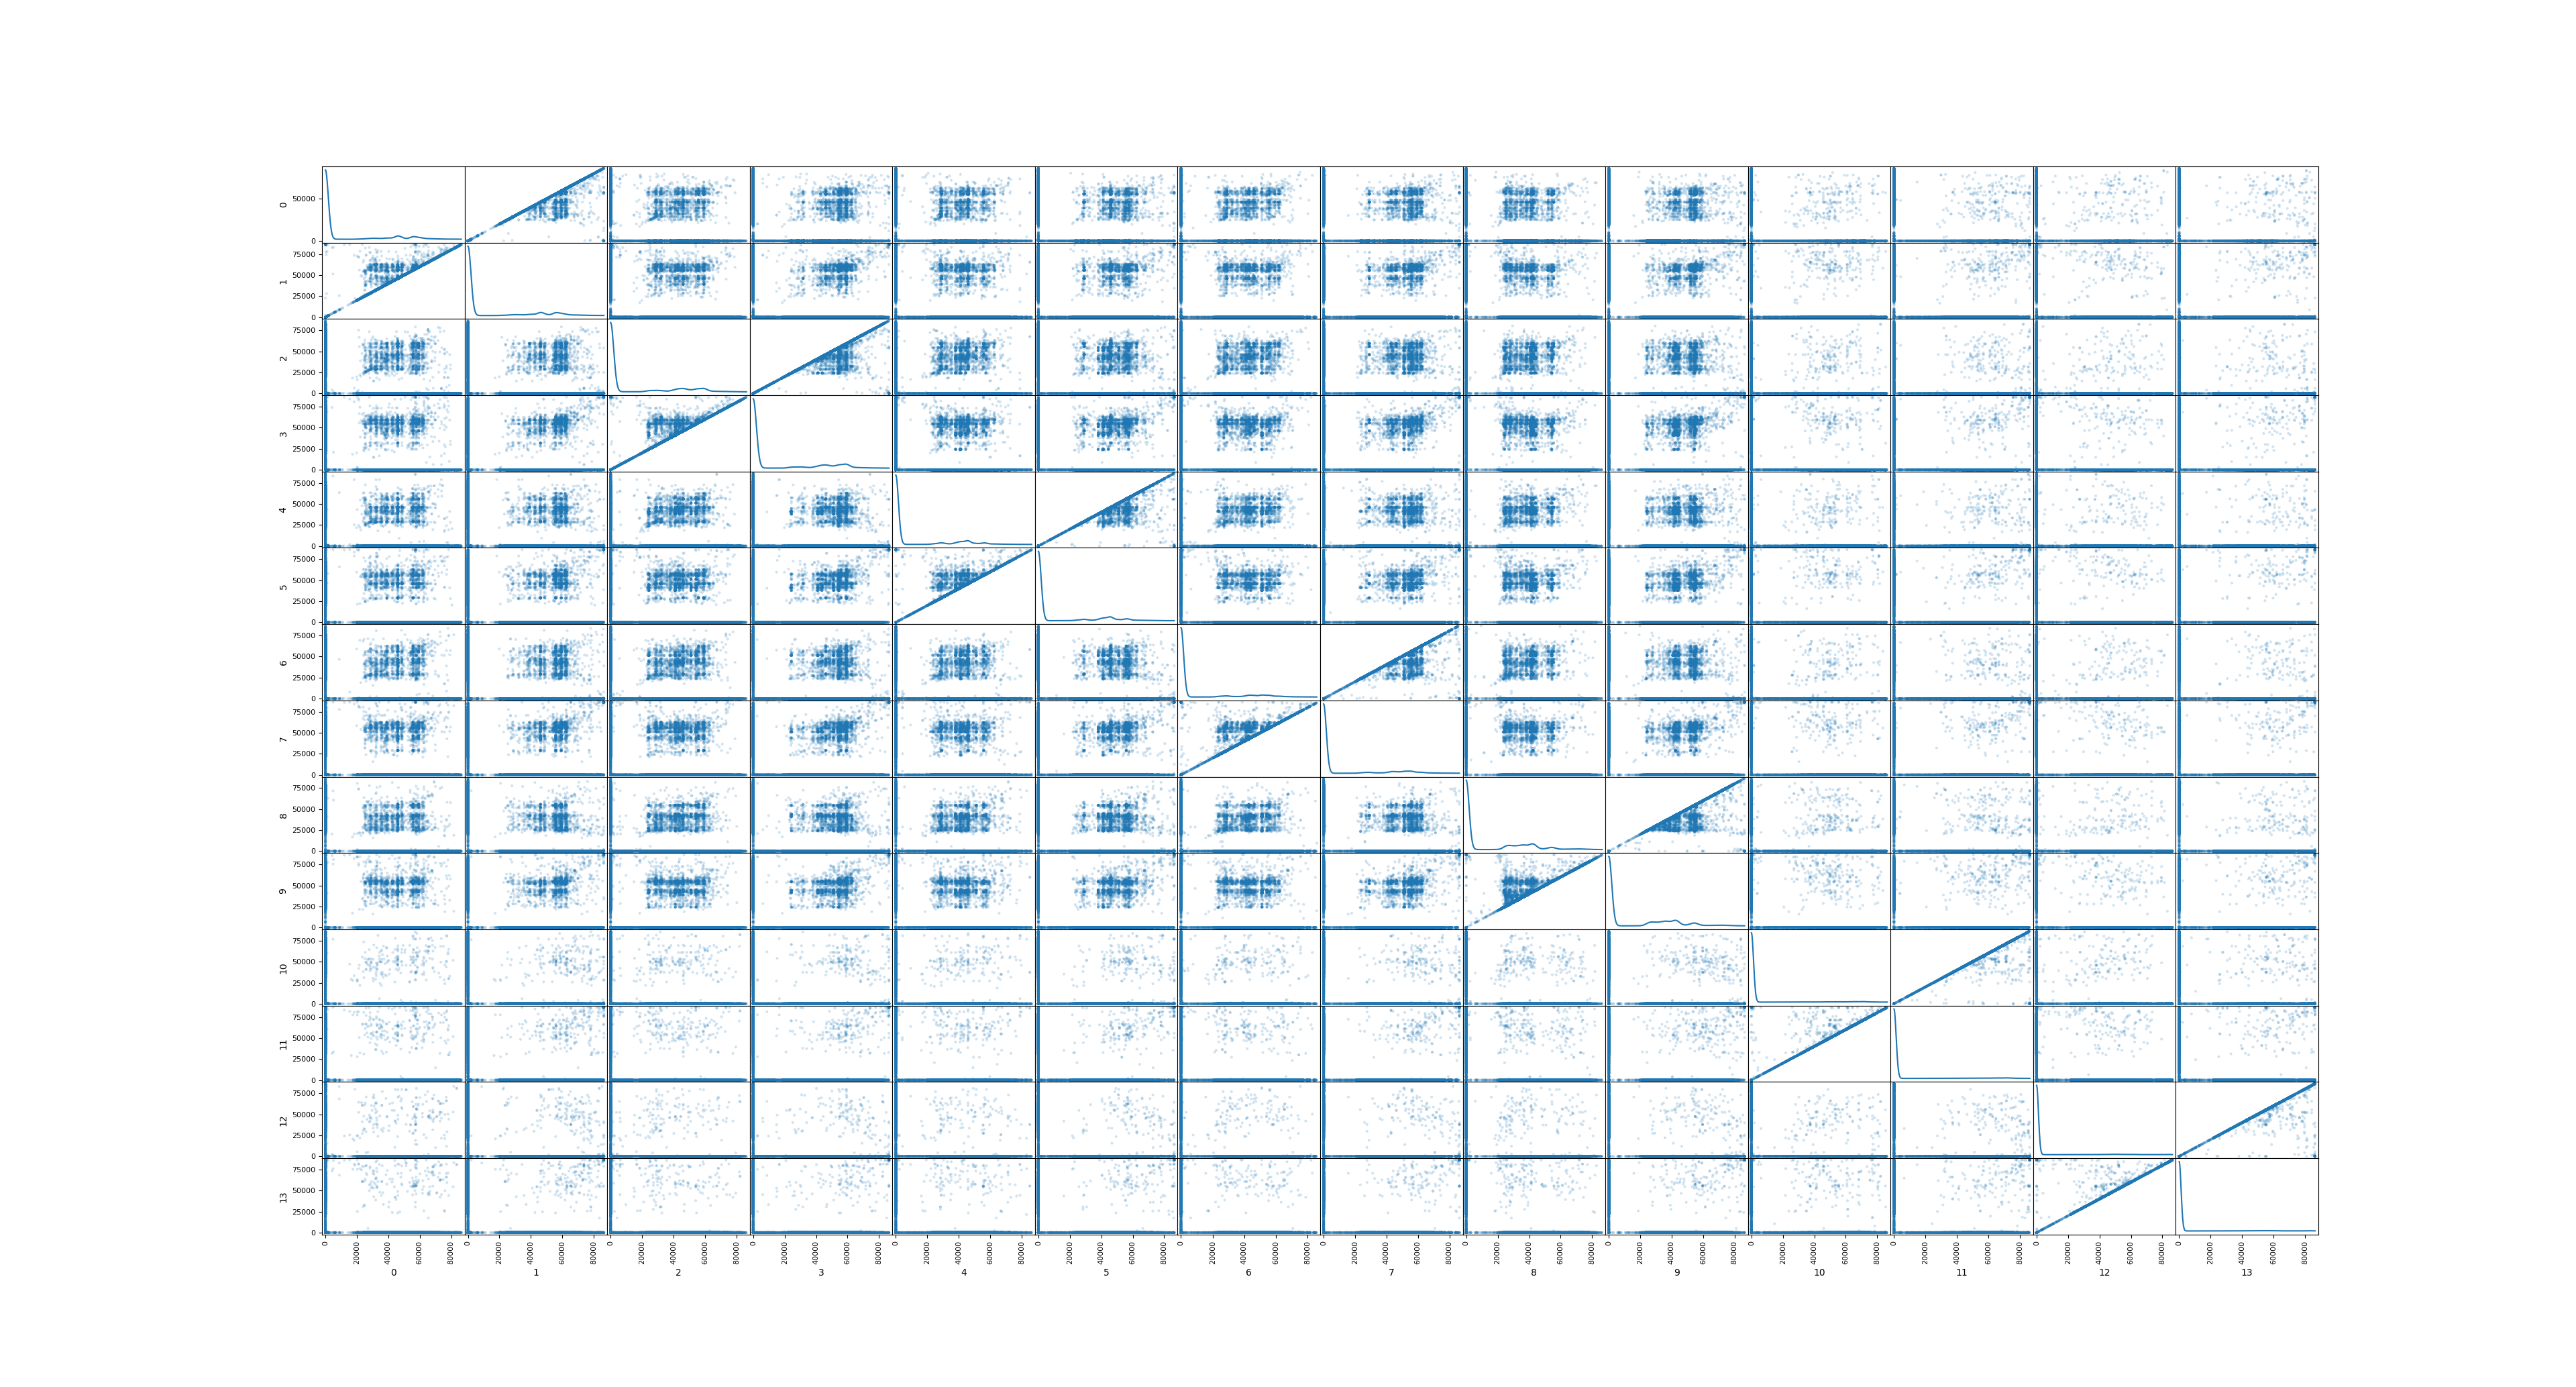
\includegraphics [width = \textwidth]{images/scattered_matrix_mean.png}
\caption{Visualization of the ten dimensions\label{fig:matrix}}
\end{figure}

Figure \ref{fig:matrix} shows the ten dimensions of my data. The weekends are clearly visible because they have less dense data points. All the lines in figure\ref{fig:matrix} visualize missing data in one way or another. Without does missing data points it shows an abstract version of the early lessons, arrival times and the last lesson, leaving time.

With the numpy array applying the different algorithms is very straight forward. Because I was not obligated to write my advanced algorithm, I used the one from sklearn. Here instead of DBSCAN it also could be meanshift or k-means. Those my have different parameters, but the rest of the code works the same. On the last line, I print the highest label number to find out the amount of groups. Depending on this, I have to change the parameters.
\begin{lstlisting}[language=Python,caption="advanced algorithm",style=python]
from sklearn.cluster import DBSCAN 
import numpy as np
X = np.load("data.npy")
db = DBSCAN(eps = 0.0075, min_samples = 1).fit(X) 
labels1 = db.labels_ 
print(max(labels1))
\end{lstlisting}

It did not matter how often I change the parameters my data was too noisy to get any real results. Cleaning up the data has the risk of losing potential students or teachers. That is why I have gone into another direction. The algorithm above is all clustering algorithms, which are supposed to find the group for themself. But I already know around which points the group should be. The K-Nearest-Neighbor (KNN) algorithm was the best option to go for, but the already provided version of the KNN was lacking the option to provide the exact location of the centroids and only calculating the distance between each MAC and the middle points.


That is why I created my own KNN algorithm. It does exactly what I said before. Usually, the distance to the expected point squared is used for the measurement. This punished long stayers and people with extra activity too much. That is why I used the sixth root out of the squared number. This ratio gave me the best results on the spectrum I could measure.
\begin{lstlisting}[language=Python, caption="own KNN",style=python]
def KNN(Y):
    p = []
    for m in c:
        l = m[1]
        d = 0
        for i in range(0,len(l)):
            if not i<len(Y):
                continue
            d+=((Y[i]-l[i])**(2))**(1/6)
        p += [(m[0],d)]
    return sorted(p,key=lambda x: x[1])
\end{lstlisting}
For the SBB algorithm I used a similar function, but only looked at the morning. There I got better results without taking the root of the distance. 

\subsection{Graphics}
For the graphics I used the famous matplotlib library in python. Especially the pyplot class from this library.
\begin{lstlisting}[language=Python, caption="graphic import",style=python]
import matplotlib.pyplot as plt
\end{lstlisting}
With this import, the rest of the code looks similar to the advanced algorithm in case of importing and getting the data. Plotting the data correctly is done with the right packets and functions from plt. The attributes provided like labeling and scale helps to make the graphics even better.

For more advanced options, this library can be used with pandas to create a scatter matrix (see Figure \ref{fig:matrix}. This gives a good visualization for multiple dimensions like my project. I use ten dimensions, which no one really can picture. With this scatter matrix, one comes close.

\begin{lstlisting}[language=Python,caption="graphic example",style=python]
from pandas.plotting import scatter_matrix
import pandas as pd
import matplotlib.pyplot as plt
X = np.load(pathtodata)
data = pd.DataFrame(X)
scatter_matrix(data,alpha=0.2, figsize=(6,6), diagonal="kde")
plt.show()
\end{lstlisting}

\subsection{Website}

I created a website to present my results and raise more awareness, then I could get only with my paper. On the website, the goal was that people in my school could find out what I know about them. I presented my findings, as discussed on the website. I used the argon2 encryption algorithm to provide brute force. Argon2 is made that I can tell them how much time it needs to encrypt. By inputting one's MAC, it gets encrypted, and with a simple dictionary lookup, it can access all of the information gathered about the person: Class, Living place, friend type (social, asocial, and so on) and username). I did not give out the username; I just said if I found it. And what I could find out only with the username, which is not necessarily legal, but easily possible.
I run a simple flask app on my server with HTML and CSS. I added also some different text for explaining how much and what information I need and the danger of Big Data and manipulation.
\begin{lstlisting}[language=Python,caption="Website sample code",style=python,label=lst:websitecode]
from flask import Flask, request, render_template, redirect,send_from_directory
app = Flask(__name__)
@app.route('/')
def home():
    return render_template('start.html',title = "Welcome")


if __name__ == "__main__":
    app.run(host="0.0.0.0", port=80)
\end{lstlisting}
In the first line of listing \ref{lst:websitecode} the needed functions from the flask library are imported. In the next line a webapp is created. Line 3-5 show a basic example that can be used to create a homepage. As soon as the address provided in line 9 is called, the function home returns the HTML page with the variable title as welcome.
The eighth line checks if this program is the original program or if it is imported into another code. If it is the main program it start the web app on line 9. To be able to access the website from other devices one has to put the host to 0.0.0.0. The port 80 is the most common used port besides the newer and more securer 443 for websites.

\section{Algorithm}
\subsection{Counting Method}
The counting method does precisely how it is called. It counts the amount of occasion of anything. Usually, there is a class that is counted as a specific MAC address or between a particular time.
\footcite{datasciencefromscratch}
\footcite[P. 289]{dataalgorithms}
\subsection{K-Nearest-Neighbor}

\begin{wrapfigure}{r}{7cm}
\centering
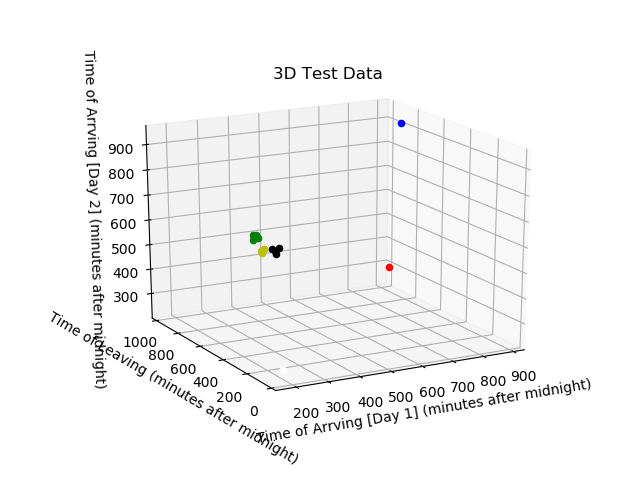
\includegraphics [width = 6cm]{images/3Dploting.png}
\caption{Simplified data example in 3D\label{fig:3dploting}}
\end{wrapfigure}

The K-Nearest-Neighbor (KNN)  is a supervised machine learning algorithm. This means it needs training data. The algorithm creates K groups by minimizing the distance to the centroids. It moves the centroids always in the direction where the error squared is reduced. In the end every point is closest to the one specific centroid. This point belongs to the group of this centroid. There are different ways to evaluate the distance. The most common used distance is the euclidean distance. It takes the sum of the distance between each point and the centroid squared and from the sum the square root.

I already had my centroids from the time table. This avoided the fact that I needed training data. The grouping to each centroid worked the same way then in the standard KNN. My algorithm had the advantage that I had complete control over my centroids and understood why this is point is order to a centroid. Also it help removing the nonstudent MAC addresses form the set or at least render them unimportant.  


\footcite{datasciencefromscratch}
\footcite[P. 305]{dataalgorithms}
\subsection{K-Means}
\begin{wrapfigure}[9]{r}{7cm}
\centering
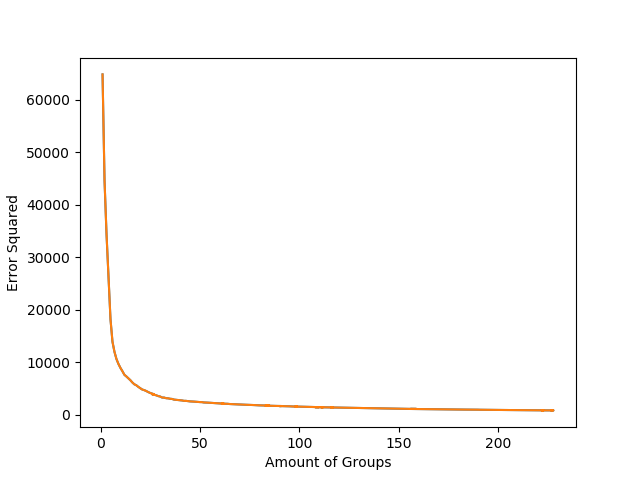
\includegraphics [width = 6cm]{images/groupstoerror.png}
\caption{Error rate declining with more data.\label{errorwithtime}}
\end{wrapfigure}
K-Means uses similar to the KNN algorithm multidimensional points in the same dimensional space. 

Unlike KNN, K-means is an unsupervised version of machine learning. That means there is no need the give any training points. This has the advantage that it can form groups without the need for labeling data. K-Means creates the K groups out of the data. It moves the centroids (the centers of the subset) around to decrease the error rate. The difficulties are to choose the number of groups correct. Figure \ref{errorwithtime} shows how the error declines when the group increases. It is essential to minimize the error rate, but too many groups are contra-productive. It is recommended to use the number of groups at the "turn".
K-means does not work well with the wrong data. It assumes that every data point is valid; therefore, it groups everything completely wrong.

\footcite{datasciencefromscratch}
\footcite{dataalgorithms}
\subsection{Descition Tree}
The decision tree is beside the counting method, the easiest to understand. It consists of several questions, and depending on the answer to these questions; it is possible to gain information. For my class example, one question could be, do you have an early lesson on Monday morning. If that is so, you belong to a category. This already excludes some of the potential classes. Repeating this step for the rest of the week, you belong to a particular subcategory with only a few potential classes left. It is called a decision tree because if drawn out, it looks similar to a tree, and at every note, one does have to make a decision. The hardest part here is to ask the right questions. Questions about the last digit of the MAC address, for example, is very pointless, and there is no information gained. The goal is to divide the groups so often in as few questions as possible, that in the end there is only one class in each group or more generally that there is only one kind of answer in a set. Not only the question matter also the right order to ask them. This can be solved simply by the computer testing the different versions and return the one with the least error and the least questions. This method did not work well for me, because it cannot evaluate error, and one wrong answer gives an entirely different solution. With more and preciser data, this could be a better way to figure out what class a person belongs to, and it is understandable, and it is also possible to remove the external or automatic nonhuman MAC-addresses and data points.
\footcite{datasciencefromscratch}
\footcite{dataalgorithms}
\subsection{DBSCAN}
DBSCAN stands for Density-Based Spatial Clustering of Application with Noise. Like the name indicates in is  a clustering algorithm, so unsupervised machine learning. This model finds dense places in a multidimensional space. From these points it expands  to create clusters of data. This should work well with similar dense data, which has a some irregularities with denser points. The most important parameter for this to work is the eps. The eps is the maximum distance between two points so they still are in the same area and could be in the same cluster or group. This does not mean that is the maximum distance between any two points of the group. With this distance you find at least one other (in a group of more then one) point in the group and when repeated one can find the whole group. 

Because this works well with equal dense room, I believed it could work with my data well. I hoped it could figure out all the times the students arrived by looking for more data at these points. But because this did not help me much and I wanted to get more information I tried to use this algorithm on my reduced data. This did not work at all. The groups created by the algorithm were seemingly random to me. \footcite{dbscan}

\subsection{Mean Shift}
Mean Shift like DBSCAN works with discovering blobs in a similar dense space. Instead of using the distance between two points to determent if the points are still in the same group, it uses centroids, like KNN and K-Means. It updates the centroids to be the mean value of the points around the centroids.\footcite{meanshift}

\[m(x_i) \frac{\sum_{x_j \in N(x_i)}K(x_j-x_i)*x_j}{\sum_{x_j \in N(x_i)} K(x_j-x_i)}\]

Here is \(x_i\) the centroid in question. \(N(x_i)\) is a function to return the samples in the neighborhood of the centroid within a given distance. m is the vector the centroid has to move to. This function calculates the weighted average of the points, weighted with the distance. 
\footcite{meanshift} \footcite{meanshiftformula}



\section{Poster}
To promote my website, although I am not proud of the design, I created several posters. I could hang them up in school all around the school. The first poster was A0 big with paper with only "Don't scan" and a QR-code on there. Another poster was a hacker with the matrix symbol and the caption "I know who you are.". I also thought about distributing a flyer. Something like a flat earth flyer, but I had no idea what text should come afterward. 

\section{Law}
The law as usually was very complexly written, but luckily for me there were some interpretation on the official Swiss governmental website. With these interpretation it is not perfect but it helped to get a descent over view and afterwards I could read in more detail the sections mentioned.

\section{How to use my code}
\begin{figure}[ht]
\centering
\begin{subfigure}[b]{0.45\linewidth}
\centering
\includegraphics[width = 0.9\linewidth]{images/git.edu-qrcode.png}
\caption{\label{fig:qredu}}
\end{subfigure}
\begin{subfigure}[b]{0.45\linewidth}
\rotatebox[origin=c]{0}{
\includegraphics[width = 0.9\linewidth]{images/qrcode_github.png}}
\centering\caption{\label{fig:qrgithub}}
\end{subfigure}
\caption{(\subref{fig:qredu}) send to the git with all the private data (only for supervisors), (\subref{fig:qrgithub}) is the link for the public code (no data).}
\end{figure}
\subsection{Preparation}
That this code works you need python, installed the repositories and you have to have a device that supports monitor mode. The last one is technically optional but it is necessary to have it for the next steps.
\subsection{Collecting data}
To be able to collect data, you need a device that you can leave at one place to sniff data and supports monitor mode. I used the WiFi pineapple tetra, which has two built-in Wi-Fi cards to sniff data on two channels at the same time (2.4GHz and 5GHz).
With the Wi-Fi pineapple, it is recommended to use an external storage device to save all the captured packets.

Depending on the device one uses, there are different scripts in the "Code/collect data" folder. I will go on with the WiFi pineapple because this is the best way (in my opinion) to do so.
There are also options for the Ngup and the software aircrack-ng.

For the WiFi pineapple, after the initial setup, one should connect to over SSH. 
If you connect via the Wi-Fi that the pineapple provides, that it is necessary to paste the WiFi pineapple.txt file content into a run.sh file on the pineapple over the terminal. 
This is necessary because the script turns off the Wi-Fi you use.

Depending on the USB stick, it needs to be first formated. Be aware that this will delete all the data on the external drive.
The code to do that is provided in the same folder with the name "formatdrive.txt".

If you choose not to use an external drive (local storage is available on the Wi-FI pineapple, but it is constrained), there is also a script ("extractdata.txt"), which provides the code to extract the data from the pineapple to the primary device.

If the possibility is there, that the pineapple my be plugged out, it helps to have the sniffing script in autostart. This helps not to lose all the files when the pineapple loses power for a short time, but there will not be a Wi-Fi from the pineapple to connect to the pineapple. One can still connect via cable to the pineapple, but it may be a little harder.

When using a USB, it is possible to unplug the USB-stick as soon as you believe in having enough data.

\subsection{First look at the data}
This step is optional to run the code and get the results.

I always took a look at my data before running the code. I used Wireshark to open the .pcap files. 
For me, the most exciting part was to find the usernames, which are sent during the handshake.
The right filter to find these usernames is in the "Code/Filtering own Data" folder under "wireshark\_filtering.txt"
In Wireshark, one can filter for other connection types or information sent. For me, it was a control that I used the right channels to capture my data.

\subsection{Parse the data}
Working with the .pcap files takes forever. There is a library that makes it possible to work with python and .pcap files.
The first thing I had to do is to reduce my data only to the MAC address and the time. I also collected usernames. Both files are in the scapy subfolder from the code folder. 
This process takes a long time. I recommend to run it in terminal not in IDLE because it uses TQDM.
After about 100 hours, about two weeks of data should be parsed. The longest part is behind us!
\subsection{How to use the data}
In the folder, an advanced algorithm contains several algorithms and ideas on how to use once data.
I created first a ten-dimensional numpy array to have to data in a uniform standard. "getdatareadyforaa\_novarianz\_meanvalue.py" creates in my experience the best results. There are other ways to do this. 
With the numpy array applying the advanced algorithm is simple. Be sure to select the right file to test and change the parameters depending on your goal and collected data.
There are several sklearn libraries used for different algorithm (mean shift,dbscan,k-means, and OPTICS)
There is also my own KNN algorithm in different versions. Some are for the classes, and some are for the SBB.

\subsection{Proof of concept code}
For proof of concept, I used the data provided by the school. The code in basic-PoC should be run with the main.py. In this program, the data location can be changed, the time-table can be modified, and the access-point data can be modified. There should be no reason to open the tools.py except to see how it is done. The help function works for every function used in the proof of concept.

\subsection{Other files on the git repositories}
\subsubsection{Arduino}
As in the paper said, I had the idea to create my own WiFi-Fpineapple. I wanted to create it with the Arduino, and in the code/arduino folder, there are a few libraries and code snippets that should make it possible to capture and sniff Wi-Fi metadata from the air.

\subsubsection{Website}
In the website folder, there are three different attends to create a website. The website\_python\_poster is the final one. To start the website, one has to run either flask run in the terminal or python3 app.py

\subsubsection{Test folder}
The test folder exists to test codes. There are a lot of subfolders with individually parsed data. Most programs have path in them which work in the text files (especially the proof of concept data)

\subsubsection{Data}
This folder is only available under the code for the supervisors.

In the data folder, I have every data point I have collected or got from the IT-department. One can run the code with this data, but one has to rewrite the code with the right path.

\subsubsection{Graphing}
In the graphing folder, it shows a few ideas on how to visualize the code one gathers. There are also testing files in there which use fake data, but for explaining the ideas, it helps a lot.

\subsubsection{Further}
There are many other programs which helped me to develop the main programs. Some of them work and are helpful, and others were no success at all. 



\section{Bibliography}
\printbibliography[title={offline},nottype={online}]

\printbibliography[title={online},type={online}]
\listoffigures
\lstlistoflistings

\end{document}